% "{'classe':('PSI'),'chapitre':'slci_stabilite','type':('cours'),'titre':'Rappels sur la détermination des performances des systèmes asservis', 'source':' ','comp':[],'corrige':True}"
\setchapterimage{Fond_SLCI.png}
\setchapterpreamble[u]{\margintoc}
%\setcounter{chapter}{1}

\chapter{Rappels sur la détermination des performances des systèmes asservis}

\marginnote[3cm]{
\UPSTIcompetence[2]{C1-01}
\UPSTIcompetence[2]{C2-03}
}

\marginnote[5cm]{\textbf{Frédéric Mazet}, \textit{Cours d'automatique de deuxième année}, Lycée Dumont Durville, Toulon.}
\marginnote[6cm]{\textbf{Florestan Mathurin}, \textit{Stabilité des SLCI}, Lycée Bellevue, Toulouse \url{http://florestan.mathurin.free.fr/}.}


\section{Stabilité des systèmes asservis}
\subsection{Notion de stabilité}
\subsubsection{Représentation graphique \cite{1}}
Un état d'équilibre d'un système est asymptotiquement stable lorsque le système, écarté de sa position d'équilibre par une
cause extérieure, finit par retrouver ce même état d'équilibre après disparition de la
cause.
Illustrons cette définition de façon très intuitive à travers l'exemple suivant : une boule
soumise à l'accélération de la pesanteur se déplaçant (avec un peu de dissipation
énergétique) sur une surface donnée.

\begin{figure}[H]
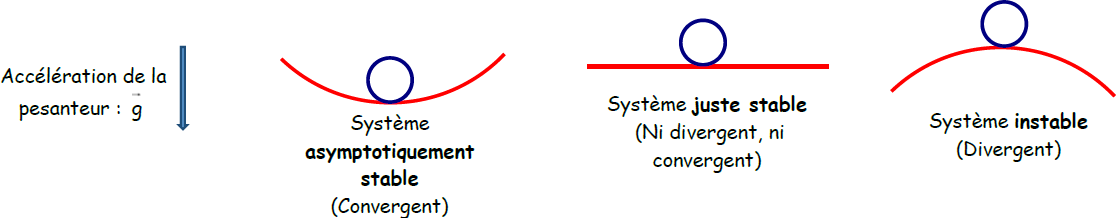
\includegraphics[width=.9\linewidth]{fig_stabilite}
\end{figure}
\subsubsection{Premières définitions}
\begin{defi}[Définition intuitive]

Un système est asymptotiquement stable si et seulement si : 
\begin{itemize}
\item abandonné à lui-même à partir de conditions initiales quelconques il revient à son état d'équilibre;
\item son régime transitoire finit par disparaître;
\item sa sortie finit par ressembler à l'entrée;
\item sa réponse tend vers zéro au cours du temps.
\end{itemize}

\end{defi}

\begin{remarque}
La stabilité d'un système \textbf{est indépendante} de la nature de l'entrée. Ainsi, l'étude de la stabilité peut se faire à partir d'une réponse impulsionnelle (entrée Dirac), indicielle (entrée échelon d'amplitude 1), d'une réponse harmonique (entrée sinusoïdale)...

Pour simplifier les calculs, une première approche pourra être d'utiliser la réponse impulsionnelle. 
\end{remarque}
\begin{defi}{}
En conséquence, on peut considérer qu'un système est asymptotiquement stable si et seulement si sa réponse impulsionnelle tend vers zéro au cours du temps.
\end{defi}

\subsubsection{Étude des pôles de la fonction de transfert}
Dans le cas général la fonction de transfert d'un système peut se mettre sous la forme :
$$
H(p)=\dfrac{b_mp^m + b_{m-1}p^{m-1}+...+b_1p+b_0}{a_np^n + a_{n-1}p^{n-1}+...+a_1p+a_0} \quad \text{avec } n\geq m.
$$

Lors du calcul de la réponse temporelle en utilisant la transformée de Laplace inverse (quelle que soit l'entrée), la nature du régime transitoire ne dépend que des pôles $p_i$de la fonction de transfert (zéros du dénominateur).

En factorisant le numérateur et le dénominateur de $H(p)$ on peut alors retrouver une fonction de la forme  :
$$
H(p)=\dfrac{\left(p+ z_m\right)\cdot \left(p+ z_{m-1}\right)...}{\left(p+ p_n\right)\cdot \left(p+ p_{n-1}\right)...} \quad \text{avec } p_i,z_i\in \mathbb{C}.
$$

En passant dans le domaine temporel : 
\begin{itemize}
\item les pôles réels (de type $p=-a$) induisent des modes \marginnote{Mode : fonction temporelle associée à un pôle.} du type $e^{-at}$;
\item les pôles complexes conjugués (de type $p=-a\pm j\omega$) induisent des modes du type 
$e^{-at} \sin \omega t$.
\end{itemize}

\textbf{On peut ainsi constater que si les pôles sont à partie réelle strictement négative, l'exponentielle décroissante permet de stabiliser la réponse temporelle.}

Ainsi, on peut observer la réponse temporelle des systèmes en fonction du positionnement des pôles dans le plan complexe. 

\begin{figure}[H]
\centering
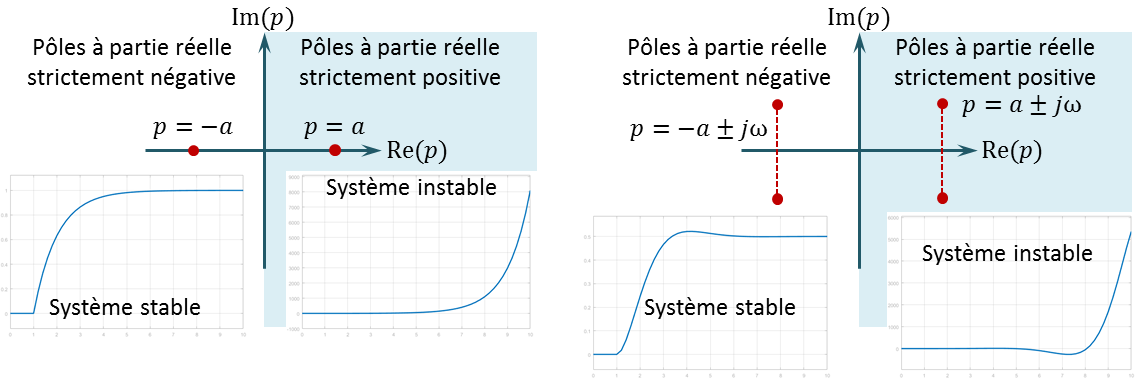
\includegraphics[width=\linewidth]{poles_simple_double}

\caption{Représentation d'un système à pôle simple et à pôles conjugués dans le plan complexe -- Réponse indicielle}
\end{figure}

\subsubsection{Position des pôles dans le plan complexe}
Par extension on peut observer dans le plan complexe les pôles de fonctions de transfert et leur indicielle associée.

\begin{figure}[H]
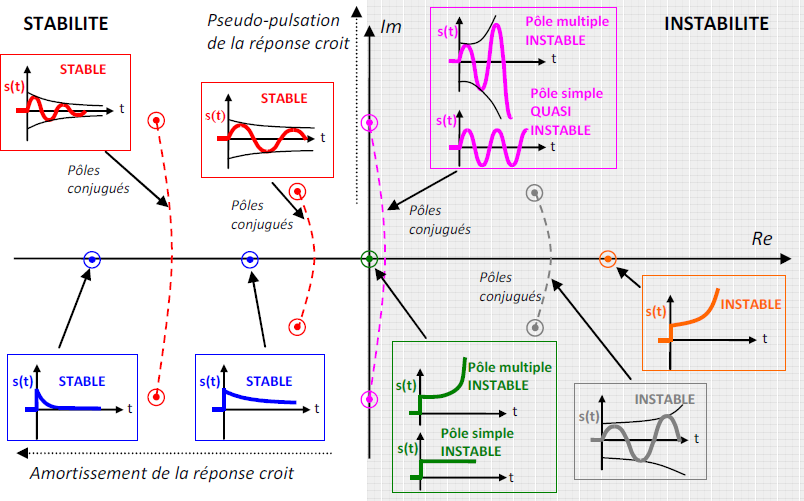
\includegraphics[width=\linewidth]{plan_complexe_fm}

\caption{Allure de la réponse à l’impulsion de Dirac selon la position des pôles de la FTBF d’un système \cite{F. Mathurin}.}
\end{figure}

\begin{defi}{À retenir}
Un système est asymptotiquement stable si et seulement si tous les pôles de sa fonction de transfert (\textbf{en boucle fermée}) sont à partie réelle strictement négative. 

\end{defi}

\begin{remarque}On peut montrer que :
\begin{itemize}
\item \textbf{pour les systèmes d'ordre 1 et 2 :} le système est stable si tous les coefficients du dénominateur sont non nuls et de même signe;
\item \textbf{pour les systèmes d'ordre 3 :} de la forme $a_0+a_1p+a_2p^2+a_3p^3$ les coefficients doivent être strictement de même signe et $a_2 a_1 > a_3 a_0$.
\end{itemize}
\end{remarque}

\subsubsection{Pôles dominants \cite{1}}
Lors de l’étude d’un système, on se contente en général de ne prendre en compte que les pôles les plus influents. Ces pôles sont appelés les pôles dominants. Pour un système asymptotiquement stable, ce sont ceux qui sont le plus proche de l’axe des imaginaires, puisque ce sont eux qui induisent des modes qui disparaissent dans le temps le plus lentement.

\subsubsection{Caractéristiques dans le lieu de pôles}
Il est possible de représenter les performances des systèmes asservis en utilisant le lieu des pôles dans le plan complexe \cite{1}. 

\subsection{Marges de stabilité}
\subsubsection{Lorsque la BO commence à pointer le bout de son nez...}



La fonction de transfert en boucle ouverte est donnée par $H_{BO}(p)=\dfrac{R(p)}{\varepsilon(p)}=F(p)G(p)$. 

\begin{marginfigure}
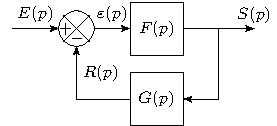
\includegraphics[width=5cm]{Schema_1_entree_F_R}
\end{marginfigure}

La fonction de transfert en boucle fermée est donnée par : $H_{BF}(p)=\dfrac{S(p)}{E(p)}=\dfrac{F(p)}{1+F(p)G(p)}=\dfrac{F(p)}{1+H_{BO}(p)}$. 

\begin{defi}[Équation caractéristique]
Soit $H(p)=\dfrac{N(p)}{D(p)}$ une fonction de transfert. On appelle $D(p)=0$ l'équation caractéristique de la fonction de transfert. Ainsi les racines de $D(p)$ correspondent aux pôles de $H(p)$.
\end{defi}

\textbf{Pour un système bouclé, l'équation caractéristique sera $1+H_{BO}(p)=0$.}

\subsubsection{Critère algébrique de stabilité : le critère de Routh}
Pour un système d'ordre supérieur à 3 il devient délicat d'obtenir analytiquement (ou numériquement) les racines du polynôme et ainsi conclure sur la stabilité à partir du signe des parties réelles. 

Il existe un critère algébrique permettant de vérifier la stabilité d'un système : il s'agit de critère de Routh. Pour un système bouclé, ce critère utilise le dénominateur de la BF. Ce critère n'étant pas au programme, on pourra rechercher dans la littérature des articles s'y référant si nécessaire. 

\subsubsection{Critère << graphique >> de stabilité : le critère du Revers}

\marginnote{
On parle ici de critère graphique car l'interprétation graphique dans le diagramme de Bode est directe.
}
 
 On a vu que l'équation caractéristique était de la forme $1+H_{BO}(p)=0$. Ainsi, Pour cela revient à résoudre l'équation $H_{BO}(p)=-1$. Ainsi dans le plan complexe, le point $(-1;0)$ permet d'avoir une information sur la stabilité. En terme de module et de phase, ce nombre complexe a un module de 1 (gain dB nul) et une phase de $-180\degres$.
 
\begin{resultat}
%Le système en boucle ouverte étant asymptotiquement stable (ou juste stable), 
Le système en boucle fermée est asymptotiquement stable si et seulement si, \textbf{en boucle ouverte, on a} :
$$
\left. G_{\text{dB}} \right|_{\omega=\omega_{-180\degres}}<0_{\text{dB}} 
\quad
\text{et}
\quad
\left. \varphi \right|_{\omega=\omega_{0\text{dB}}}>-180\degres.
$$

En notant $\omega_{-180\degres}$ la pulsation pour laquelle la phase vaut $-180\degres$ et $\omega_{0\text{dB}}$ la pulsation pour laquelle le gain est nul.
\end{resultat}
 
 
\begin{resultat}
Condition (non suffisante ...) de stabilité : les pôles de la FTBO doivent être à partie réelle positive.
\end{resultat}
 
\begin{center}
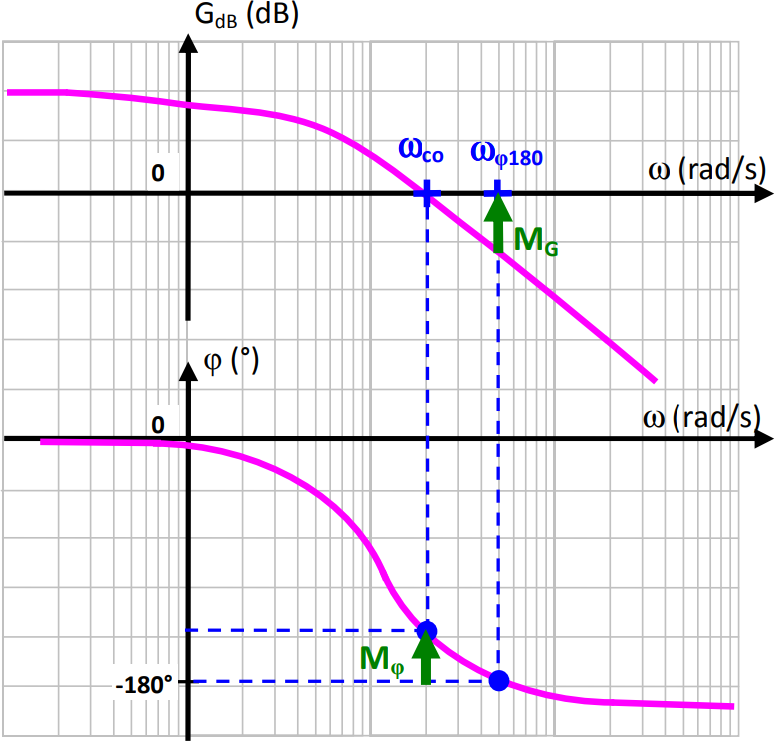
\includegraphics[width=.9\linewidth]{marges}
\end{center} 
\subsubsection{Vers le système réel...}

Le résultat donné ci-dessus est un résultat théorique dans le sens ou le diagramme de Bode de la boucle ouverte du système réel aura un écart avec le diagramme de Bode du système modélisé. 


\begin{resultat}[Marges]
Pour tenir compte des écarts entre le modèle et le système réel, on est amené à définir une marge de gain et une marge de phase. Cela signifie que dans l'étude des systèmes asservis, on considèrera, dans le cas général que le système est stable si :
\begin{itemize}
\item la marge de gain est supérieure à \SI{10}{dB};
\item la marge de phase est supérieure à $45\degres$.
\end{itemize}
\end{resultat}

\begin{marginfigure}
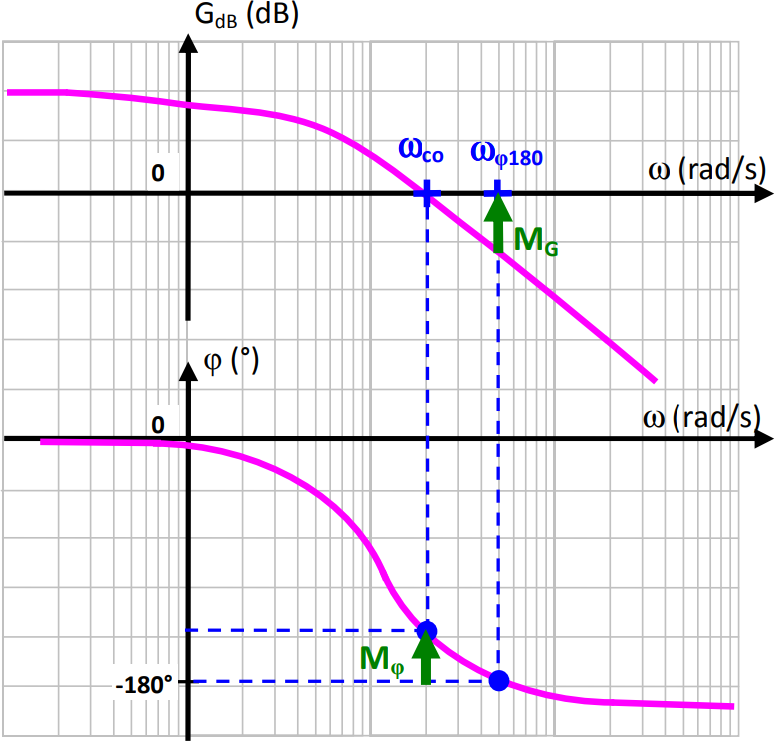
\includegraphics[width=\linewidth]{marges_fm}
\end{marginfigure}

\begin{defi}[Marge de phase]
La marge de phase est définie telle que $M_\varphi= \SI{180}{\degree} + \arg\left(\text{FTBO}(j\omega_{\text{c0}})\right)$ où $\omega_{\text{c0}}$ est la pulsation de coupure pour laquelle $20\log|\text{FTBO}\left(j\omega_{\text{c0}}\right)|=\SI{0}{dB}$.
\end{defi}

\begin{defi}[Marge de gain]
La marge de gain est définie telle que $M_G = -20\log|\text{FTBO} (j\omega_{\varphi 180})|$
où $\omega_{\varphi 180}$ est la pulsation pour laquelle $\arg(\text{FTBO}(j\omega_{ \varphi 180}))= -\SI{180}{\degres}$.
\end{defi}



 
La marge de gain permet compte de tenir compte de variations de gain de la boucle ouverte. 

De même, la marge de phase permet de tenir compte de variation de phase (retard ou déphasage non modélisés). 

La nécessité d'avoir recours à des marges de stabilité apparaît notamment lorsque : 
\begin{itemize}
\item la simplification du modèle amène à considérer uniquement les pôles dominant, 
\item le modèle ne prend pas en compte la dynamique de certains composants du système;
\item le système n'est pas invariant au cours du temps;
\item on s'éloigne de la zone de fonctionnement linéaire;
\item certaines non linéarités sont ignorées.
\end{itemize}

%\begin{thebibliography}{2}
%   \bibitem{mazet_autom} 
%   Frédéric Mazet, Cours d'automatique de deuxième année, Lycée Dumont Durville, Toulon.
%   \bibitem{mathurin_stabilite} 
%   Florestan Mathurin, Stabilité des SLCI, Lycée Bellevue, Toulouse, \url{http://florestan.mathurin.free.fr/}.
%\end{thebibliography}

